% !TeX root = simplesnt-doc.tex
\documentclass{simplesnt}

%% Helpful packages
\usepackage{simplebnf}[2023/11/25]
\usepackage{kotex}
\usepackage{xcolor}
\usepackage{amsmath,amssymb}
\usepackage{amsfonts}
\usepackage{tikz}
\usetikzlibrary{calc}
\usepackage{siunitx}
\usepackage{caption}
\usepackage{listings}
\usepackage{mathrsfs}
\usepackage{stmaryrd}
\usepackage{subcaption}
\usepackage{graphicx}


\captionsetup{font=small}
\lstset{basicstyle = \small\ttfamily, breaklines}

\usepackage{tabularray}
\UseTblrLibrary{booktabs}

\usepackage{metalogo}
\usepackage{kotex-logo}


\newcommand{\textalt}[2]{#1\textsubscript{\ensuremath{\text{\scriptsize\textit{#2}}}}}
\newcommand*{\presentfont}[1]{{\fontspec{#1}#1}}
\ExplSyntaxOn
\bool_if:nF { \sys_if_engine_xetex_p: || \sys_if_engine_luatex_p: }
  { \newcommand*{\fontspec}[1]{} }
\ExplSyntaxOff
\newfontfamily\terminalfont{Consolas}

\title{Big-Step 증명나무 합성으로 분석기 골탕먹이기}
\author{정원준}

\begin{document}
\date{2026년 5월 15일}
\maketitle


\begin{frame}
  \frametitle{목차}
  \tableofcontents
\end{frame}



\section{정적 분석기의 부정확성}
\begin{frame}[c, fragile]
  \frametitle{정적 분석이란?}

  \setlength{\columnsep}{16pt}

  \begin{columns}[T,onlytextwidth]
    \column{0.46\textwidth}
    \hfill
    \begin{minipage}{0.78\linewidth}
    \lstset{
      language=Python,
      basicstyle=\ttfamily\small,
      lineskip=2pt,
      columns=fullflexible,
      escapeinside={(*@}{@*)},
    }
    \begin{lstlisting}
x = 1
while x < 10000:
    (*@\textcolor{red}{x = x + 1}@*)
print(x)
    \end{lstlisting}
    \end{minipage}

    \column{0.54\textwidth}
    \vspace{8pt}
    \begin{itemize}
      \item<2-> x가 어떤 값을 가질 수 있을까?
      \item<3-> x가 특정 위치에서 어떤 값을 가질 수 있을까?
      \item<4-> 프로그램을 돌려보지 않고 미리 알 수는 없을까?
      \item<5-> \textcolor{red}{완벽하게 알 수는 없음!}
      \item<6-> ``Rice's Theorem''
    \end{itemize}
  \end{columns}

\end{frame}
\begin{frame}[fragile]
  \frametitle{넓게 어림잡기}

  \begin{center}
    \begin{minipage}{0.34\linewidth}
      \begin{lstlisting}[basicstyle=\small\ttfamily, escapeinside={(*@}{@*)}]
if x > 0:
    x = 3
else:
    x = -3
(*@\texttt{print(x)}@*)
      \end{lstlisting}
    \end{minipage}
  \end{center}

  \vspace{12pt}

  \begin{center}
    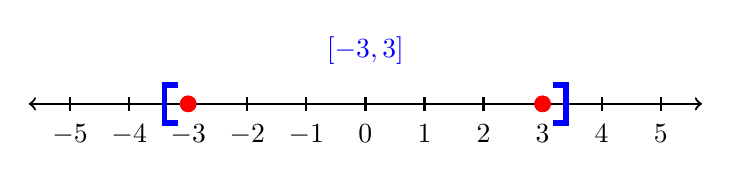
\begin{tikzpicture}[x=0.75cm, y=0.75cm]
      \draw[<->, thick] (-5.7,0) -- (5.7,0);
      \foreach \x in {-5,-4,...,5} {
        \draw[thick] (\x,0.12) -- (\x,-0.12);
        \node[below] at (\x,-0.18) {\(\x\)};
      }
      \uncover<2->{
        \fill[red] (-3,0) circle (3pt);
        \fill[red] (3,0) circle (3pt);
      }
      \uncover<3->{
        \draw[blue, line width=2pt]
          (-3.18,-0.32) -- (-3.4,-0.32) -- (-3.4,0.32) -- (-3.18,0.32);
        \draw[blue, line width=2pt]
          (3.18,-0.32) -- (3.4,-0.32) -- (3.4,0.32) -- (3.18,0.32);
        \node[blue, above] at (0,0.5) {\([ -3, 3 ]\)};
        \fill[red] (-3,0) circle (3pt);
        \fill[red] (3,0) circle (3pt);
      }
    \end{tikzpicture}
  \end{center}
\end{frame}

\begin{frame}[fragile]
  \frametitle{공격 프로그램의 예시}

  \begin{center}
    \begin{minipage}{0.34\linewidth}
      \begin{visibleenv}<2->
      \begin{lstlisting}[basicstyle=\small\ttfamily, escapeinside={(*@}{@*)}]
if x > 0:
    x = 3
else:
    x = -3
(*@\only<2>{\texttt{print(x)}}\only<3->{\textcolor{red}{\texttt{y = 10 / x}}}@*)
      \end{lstlisting}
      \end{visibleenv}
    \end{minipage}
    \makebox[0pt][l]{\hspace{16pt}\visible<3->{\textcolor{red}{false alarm 발생}}}
  \end{center}

  \vspace{12pt}

  \begin{visibleenv}<2->
    \begin{center}
      \begin{tikzpicture}[x=0.75cm, y=0.75cm]
        \draw[<->, thick] (-5.7,0) -- (5.7,0);
        \foreach \x in {-5,-4,...,5} {
          \draw[thick] (\x,0.12) -- (\x,-0.12);
          \node[below] at (\x,-0.18) {\(\x\)};
        }
        \fill[red] (-3,0) circle (3pt);
        \fill[red] (3,0) circle (3pt);
        \draw[blue, line width=2pt]
          (-3.18,-0.32) -- (-3.4,-0.32) -- (-3.4,0.32) -- (-3.18,0.32);
        \draw[blue, line width=2pt]
          (3.18,-0.32) -- (3.4,-0.32) -- (3.4,0.32) -- (3.18,0.32);
        \node[blue, above] at (0,0.5) {\([ -3, 3 ]\)};
        \fill[red] (-3,0) circle (3pt);
        \fill[red] (3,0) circle (3pt);
        \only<3->{
          \draw[red, line width=1.5pt] (0,0) circle (3pt);
        }
        \only<4->{
          \node[overlay, below] at (0,-1.0)
            {이런 공격을 일반적인 분석기에 대해서 하는 것이 목표};
        }
      \end{tikzpicture}
    \end{center}
  \end{visibleenv}
\end{frame}
\begin{frame}
  \frametitle{공격의 기대효과}
  \begin{itemize}
    \item<2-> 분석기의 약점을 파악하고 강화하는 가이드라인으로 사용
    \item<3-> 분석이 잘 안 되는 코드 조각을 삽입해서 난독화로 사용
  \end{itemize}
\end{frame}

\section{프로그램 합성과 증명나무 합성} %공격 성공 보장도 여기서 설명
\begin{frame}
  \frametitle{프로그램 합성}
  \begin{itemize}
    \item 주어진 성질을 만족하는 프로그램을 자동으로 생성!
    \item ``입력이 1, 2, 3, 4일 때 각각 1, 3, 6, 10이 나오는 프로그램을 만들어 줘'' -> (코드)
    \item ``입력이 $x$이고 출력이 $y$일 때, $y^2 \le x < (y+1)^2$가 되는 프로그램을 만들어 줘'' -> (코드)
  \end{itemize}
\end{frame}
\begin{frame}
  \frametitle{프로그램 합성}
  \begin{itemize}
    \item 정답이 있는 문제의 경우
    \item bottom-up enumeration을 통해 유한 시간 안에 끝남을 보장할 수 있음
    \item 모든 가능한 프로그램을 빠짐없이 검사 -> 여러 가지 트릭으로 시간 단축
  \end{itemize}
\end{frame}


\begin{frame}
  \frametitle{분석기 골탕먹이기 문제}
  \begin{itemize}
    \item ``분석기가 false alarm을 내는 프로그램을 만들어 줘''
    \item Rice's Theorem 덕분에 정답이 있음을 보장
    \item 그렇다면 전탐색으로 쉽게 유한 시간 안에 풀 수 있겠네?
    \item \textcolor{red}{No.} false alarm이 진짜 나는지 알 방법이 없음
  \end{itemize}
\end{frame}

\begin{frame}
  \frametitle{증명나무 합성}
  \begin{itemize}
    \item 프로그램의 ``진짜'' 실행 의미를 알 수 없다는 게 문제
    \item 어떻게 하면 프로그램을 합성할 때 실행 의미까지 같이 끌고 다닐 수 있을까?
    \item 프로그램의 실행 의미를 Big-Step으로 정의해서 그 증명나무를 합성해보자
  \end{itemize}
\end{frame}

\begin{frame}[fragile]
  \frametitle{증명나무 합성 예시}

  \begin{center}
    \begin{minipage}{\textwidth}
      \begin{lstlisting}[basicstyle=\tiny\terminalfont, columns=fixed]
                         ----------------   ----------------
                         {x: 1} |- x => 1   {x: 1} |- 1 => 1
                         -----------------------------------
     ------------              {x: 1} |- (x < 1) => 0       
     {} |- 1 => 1        -----------------------------------
----------------------   {x: 1} |- while (x < 1)  => {x: 1} 
{} |- x := 1 => {x: 1}               x := (x + 1)           
------------------------------------------------------------
               {} |- x := 1;        => {x: 1}               
                     while (x < 1)                          
                       x := (x + 1)
      \end{lstlisting}
    \end{minipage}
  \end{center}
\end{frame}

\section{증명나무 합성 디테일}
\begin{frame}
  \frametitle{증명나무 합성 디테일}
  \begin{itemize}
    \item size 정의가 왜 중요한가, 2차원 size 순서 정렬
    \item 프로그램 합성과 다르게 짝짜꿍이 잘 맞아야 됨
    \item environment 제한
    \item proof tree가 아닌 일반 코드 조각도 합성해야 함
    \item pruning 방법, ``분석기 존중''의 정의, 프로그램 합성에서의 pruning과 어떻게 다른지
  \end{itemize}
\end{frame}

\section{결과}
\begin{frame}
  \frametitle{결과}
  \begin{itemize}
    \item 첫번째 결과 설명: while 0 처리 안됨
    \item 두번째 결과 설명: interval widening
    \item 분석기가 굉장히 약한 걸로 시작해서, 합성기와 평행하게 같이 강해지기
  \end{itemize}
\end{frame}

\section{앞으로 할 일}
\begin{frame}
  \begin{itemize}
    \item ``좋은 proof tree 조각'' 평가 휴리스틱
    \item bottom up은 너무 많은 코드/증명 조각을 생성함. 좋은 쪽으로 많이 생성하려면?
    \item ``좋은 공격''이 뭔지 계속 다듬으면서 생각하기
    \item pruning
    \item llm guide
    \item ``비슷한 공격''들을 많이 제시해주는 건 의미가 없음. 비슷한 걸 거르고 다양하게 결과를 내주려면?
  \end{itemize}
\end{frame}



% 감사합니다

\definecolor{mydarkblue}{RGB}{32,56,61}

\setbeamercolor{background canvas}{bg=mydarkblue}
\setbeamercolor{normal text}{fg=white}
\setbeamercolor{frametitle}{fg=white}
\addtocounter{framenumber}{-1} % 마지막 슬라이드 번호를 하나 줄임
\appendix
\begin{frame}[c] % [c]는 내용 수직 가운데 정렬
  \centering
  {\Large \textcolor{white}{감사합니다}}
\end{frame}

\end{document}
